%%%%%%%%%%%%%%%%%%%%%%% file template.tex %%%%%%%%%%%%%%%%%%%%%%%%%
%
% This is a general template file for the LaTeX package SVJour3
% for Springer journals.          Springer Heidelberg 2010/09/16
%
% Copy it to a new file with a new name and use it as the basis
% for your article. Delete % signs as needed.
%
% This template includes a few options for different layouts and
% content for various journals. Please consult a previous issue of
% your journal as needed.
%
%%%%%%%%%%%%%%%%%%%%%%%%%%%%%%%%%%%%%%%%%%%%%%%%%%%%%%%%%%%%%%%%%%%
%
% First comes an example EPS file -- just ignore it and
% proceed on the \documentclass line
% your LaTeX will extract the file if required
% \begin{filecontents*}{example.eps}
%!PS-Adobe-3.0 EPSF-3.0
%%BoundingBox: 19 19 221 221
%%CreationDate: Mon Sep 29 1997
%%Creator: programmed by hand (JK)
%%EndComments
% gsave
% newpath
%   20 20 moveto
%   20 220 lineto
%   220 220 lineto
%   220 20 lineto
% closepath
% 2 setlinewidth
% gsave
%   .4 setgray fill
% grestore
% stroke
% grestore
% \end{filecontents*}
%
\RequirePackage{fix-cm}

%
%\documentclass{svjour3}                     % onecolumn (standard format)
%\documentclass[smallcondensed]{svjour3}     % onecolumn (ditto)
\documentclass[smallextended]{svjour3}       % onecolumn (second format)
%\documentclass[twocolumn]{svjour3}          % twocolumn
%
\smartqed  % flush right qed marks, e.g. at end of proof
%
\usepackage{graphicx}
%
% \usepackage{mathptmx}      % use Times fonts if available on your TeX system
%
% insert here the call for the packages your document requires
\usepackage[authoryear]{natbib}
\usepackage{siunitx}
\usepackage{hyperref}
\usepackage{lineno}
\usepackage{setspace}
\usepackage{booktabs}
\usepackage{longtable}
% \usepackage[utf8]{inputenc}
\doublespacing
%\usepackage{latexsym}
% etc.
%
% please place your own definitions here and don't use \def but
% \newcommand{}{}
%
% Insert the name of "your journal" with
\journalname{Estuaries and Coasts}
%
\begin{document}
\linenumbers

\title{Fine-scale relationships between phytoplankton abundance and environmental drivers in Florida Bay, USA%\thanks{Grants or other notes
%about the article that should go on the front page should be
%placed here. General acknowledgments should be placed at the end of the article.}
}
% \subtitle{Do you have a subtitle?\\ If so, write it here}

\titlerunning{Fine-scale phytoplankton abundance in Florida Bay}        % if too long for running head

\author{Joseph Stachelek         \and
        Christopher J. Madden  \and
        Stephen Kelly \and
        Michelle Blaha
}

%\authorrunning{Short form of author list} % if too long for running head

\institute{J. Stachelek \at
              South Florida Water Management District \\
              Everglades Systems Assessment Section \\
              West Palm Beach, FL 33406, USA \\
              \email{stachel2@msu.edu}             \\
              \emph{Present address:} of J. Stachelek  %  if needed
            \at
              Michigan State University \\
              East Lansing, MI, 48824, USA
}

\date{Edited: 2017-08-04 / Received: date / Accepted: date}
% The correct dates will be entered by the editor


\maketitle

\section{Appendix}

Interpolated chlorophyll estimates were quantitatively checked against independent DBHYDRO chlorophyll concentrations (Table A1). However, the timing of these measurements did not exactly match the dates of Dataflow surveys. We restricted our quantitative comparisons to surveys when DBHYDRO samples were collected within 4 days from the date of a Dataflow survey. This four day window was chosen because the temporal autocorrelation of salinity data from USGS platforms (Trout Creek) decreases markedly beyond a 3 day lag (Figure A1).

With the exception of October 2009, the root mean squared error of chlorophyll concentration estimates were less than 1 µg/L (Table A1). The coefficient of determination (R2) values are low for DBHYDRO versus Dataflow estimated chlorophyll. However, this is a symptom of the low range of chlorophyll concentration. This range is small enough that temporal mismatch (variability) and measurement error are at least as large as the spatial chlorophyll variability.

Chlorophyll maps presented throughout this paper represent the mean prediction from multiple linear regressions using the coefficients presented in Table 2. Figure A2 shows an example of the variation in output between the lower and upper 95\% prediction intervals. Figure A3 and A4 show spatial variation within individuals basins of Florida Bay. There is an indication of a higher chlorophyll "hotspot" in western Joe Bay in 2009, 2013, and 2015 (Figure A3). In addition, there in indication of the scale at which the "plume" from Taylor River extends into Little Madeira Bay (Figure A4).

\newpage

Table A1: Quantitative validation of chlorophyll concentration estimates against independent measurements from the DBHYDRO database. R2 = coefficient of determination, RMSE  = root-mean-squared error, PE = percent error, logmse = log mean-squared error.

\begin{longtable}[c]{@{}llllll@{}}
\toprule
Surveys & Days & R2 & RMSE & PE & logmse\tabularnewline
\midrule
\endhead
2009-10 & 3.83 & 0.10 & 3.54 & 77.94 & 2.53\tabularnewline
2010-07 & 1.04 & 0.40 & 0.34 & 104.51 & -2.17\tabularnewline
2011-05 & 3.74 & 0.34 & 0.40 & 361.37 & -1.86\tabularnewline
2012-06 & 3.07 & 0.13 & 0.74 & 64.37 & -0.60\tabularnewline
2012-12 & 3.10 & 0.85 & 0.59 & 92.87 & -1.05\tabularnewline
2014-07 & 1.85 & 0.30 & 0.38 & 211.86 & -1.93\tabularnewline
\bottomrule
\end{longtable}

\newpage

\begin{figure*}
  \centering
  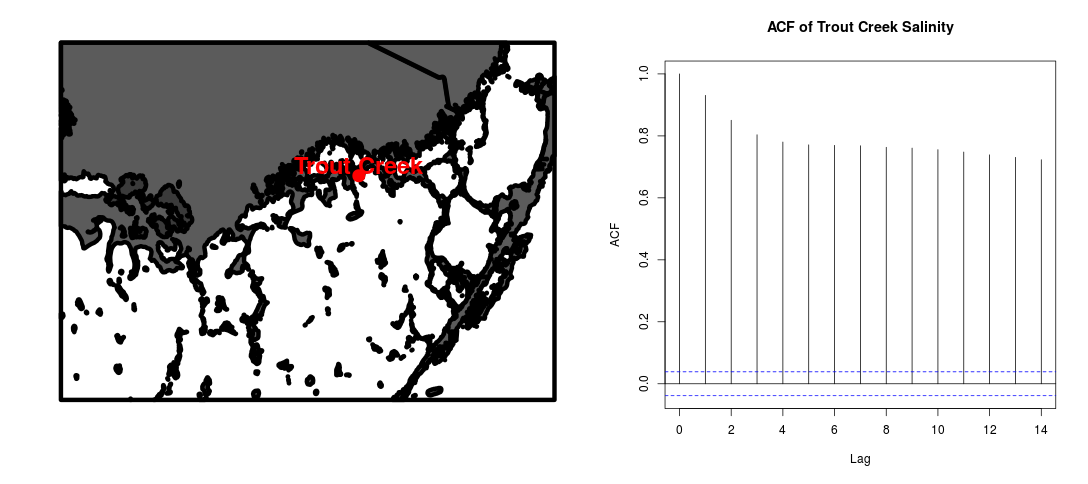
\includegraphics[width=0.75\textwidth]{../../figures/trout.png}
  \caption{left) Representative track line of a Dataflow survey (September 2015) and location of United States Geological Survey Trout Creek monitoring station \#251253080320100. right) Autocorrelation function of Trout Creek salinity.}
  \label{fig:a1}
\end{figure*}

\begin{figure*}
  \centering
  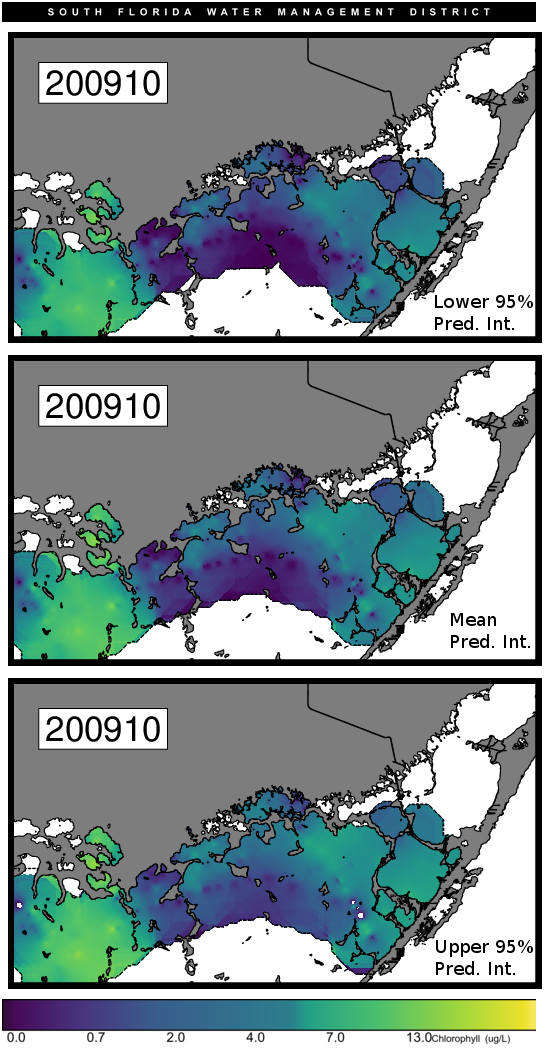
\includegraphics[width=0.75\textwidth]{../../figures/200910_chl-sefit.png}
  \caption{Example of 95\% prediction standard errors relative to the mean for October 2009.}
  \label{fig:a2}
\end{figure*}

\begin{figure*}
  \centering
  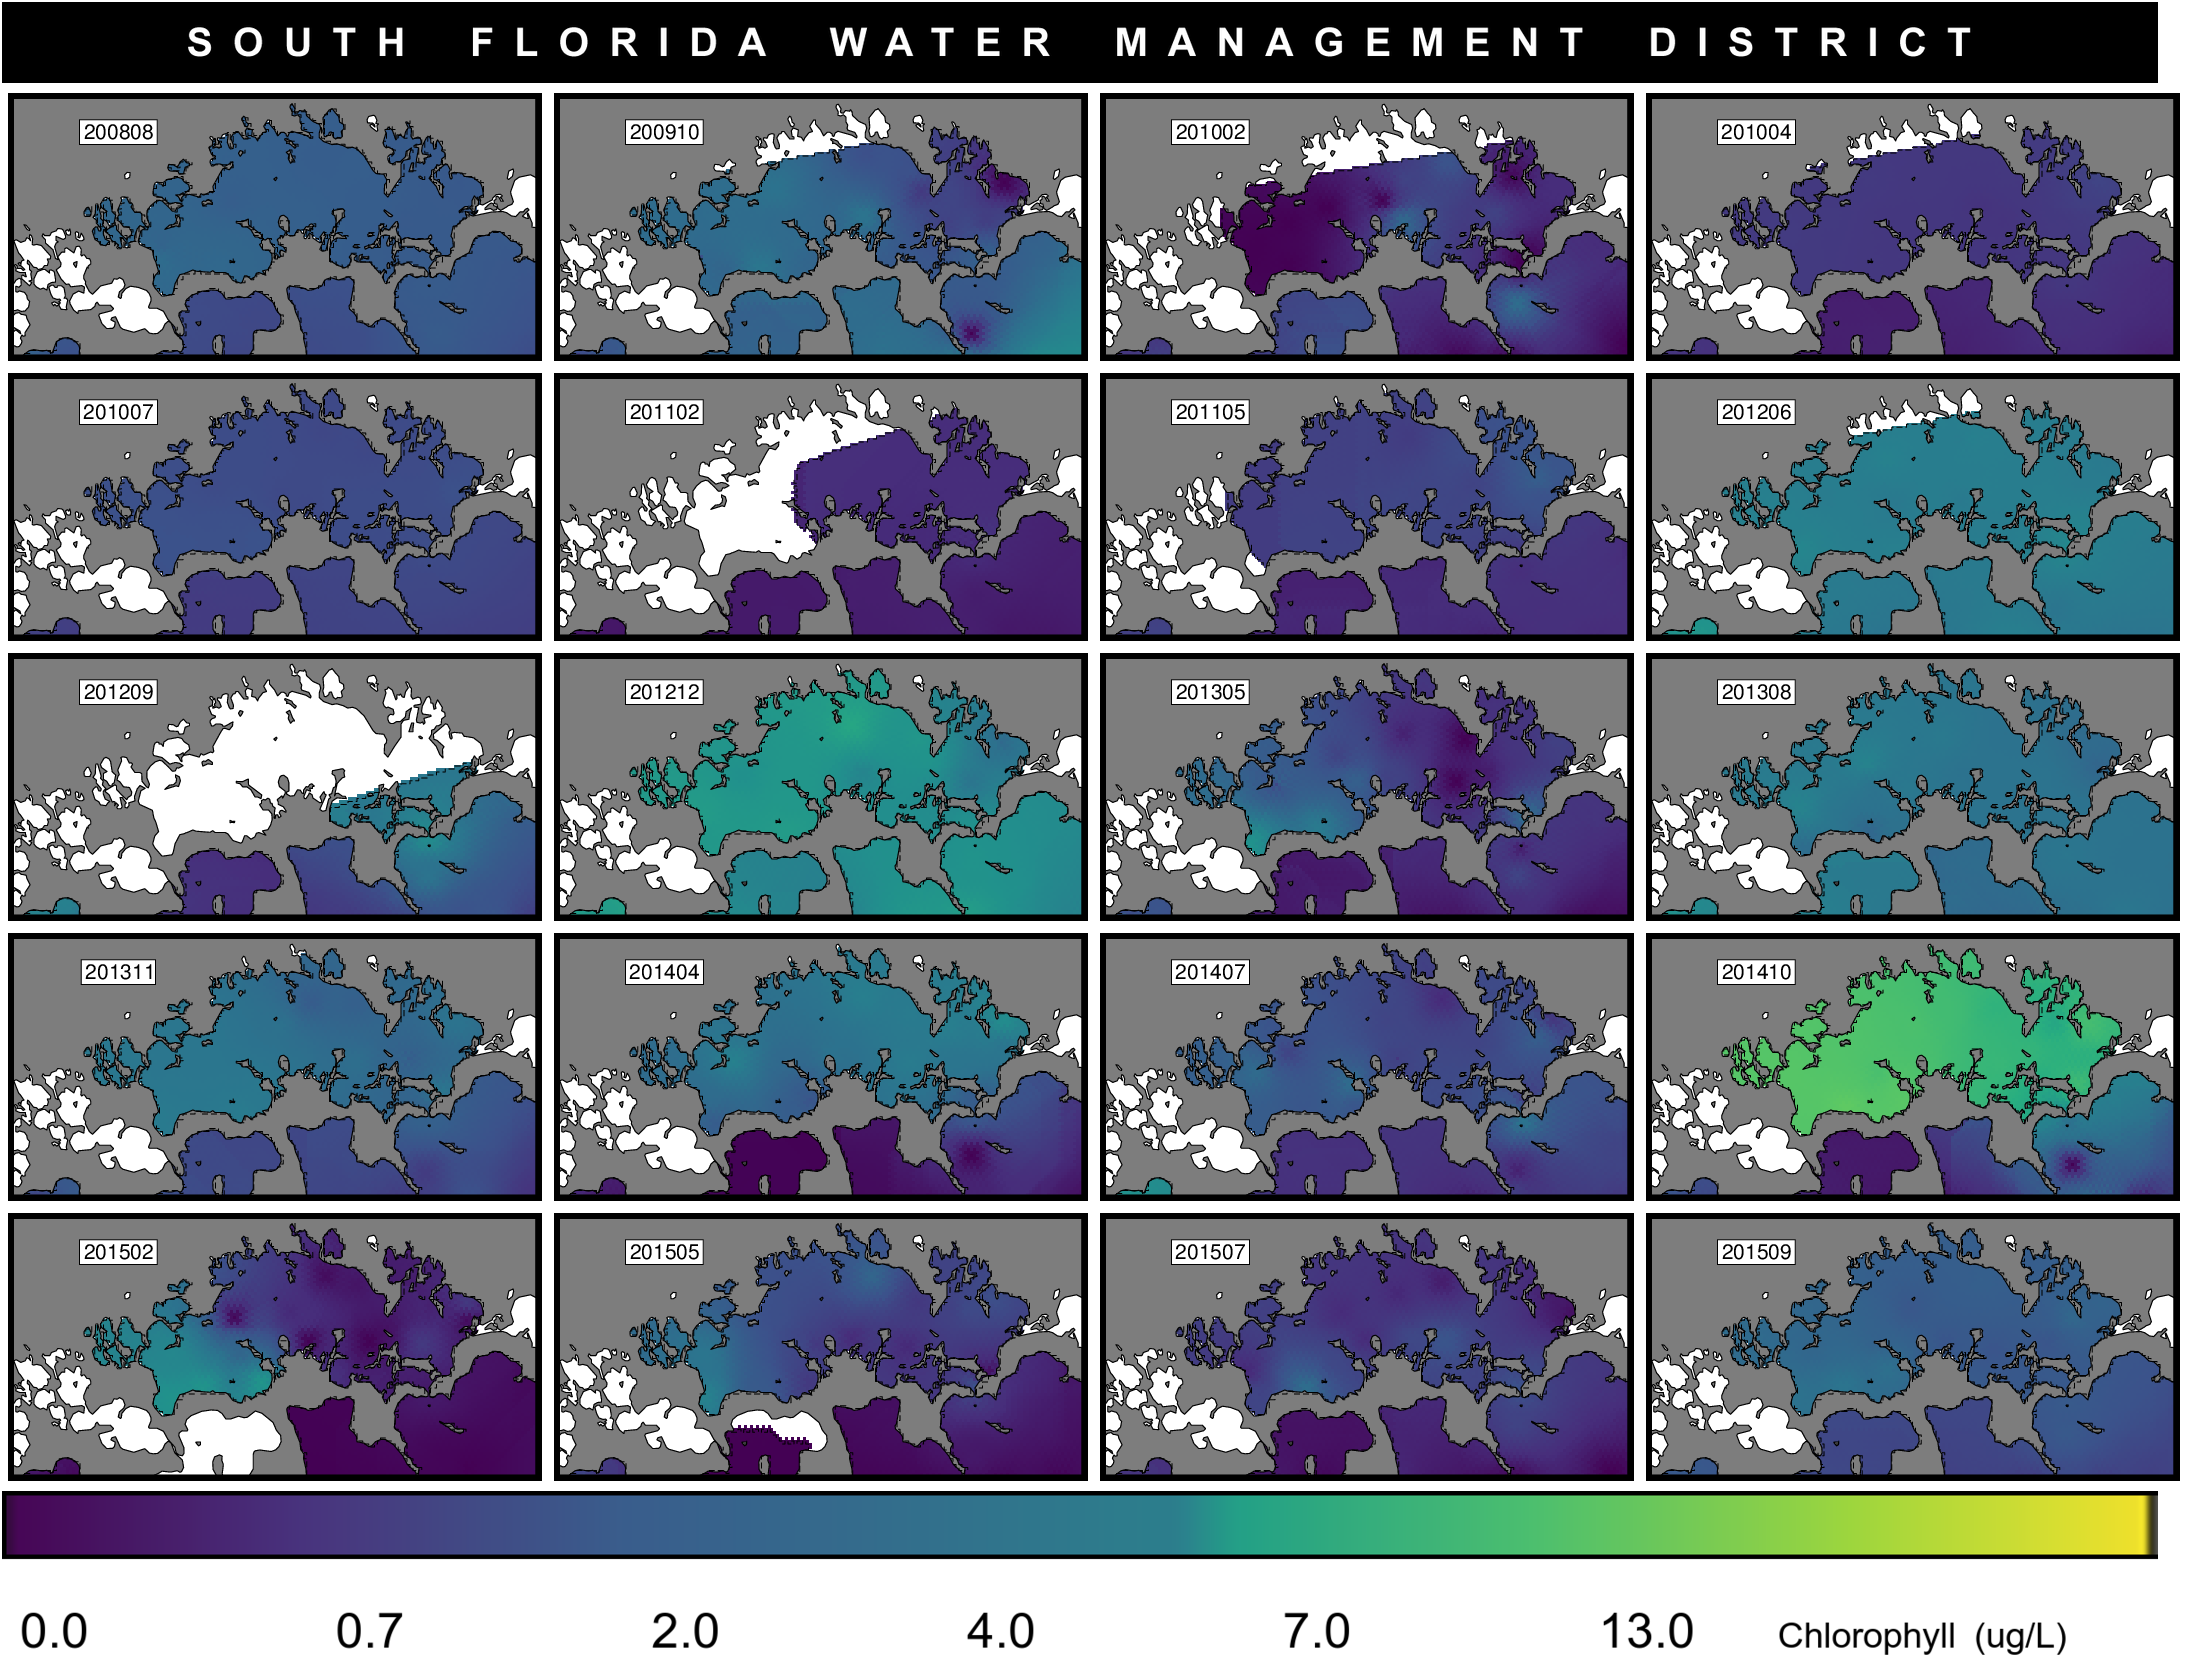
\includegraphics[width=0.75\textwidth]{../../figures/multipanel_jb.png}
  \caption{Chlorophyll concentration in Joe Bay calculated from multiple linear regression using the coefficients in Table 1. Note that the color ramp is log-scaled.}
  \label{fig:a3}
\end{figure*}

\begin{figure*}
  \centering
  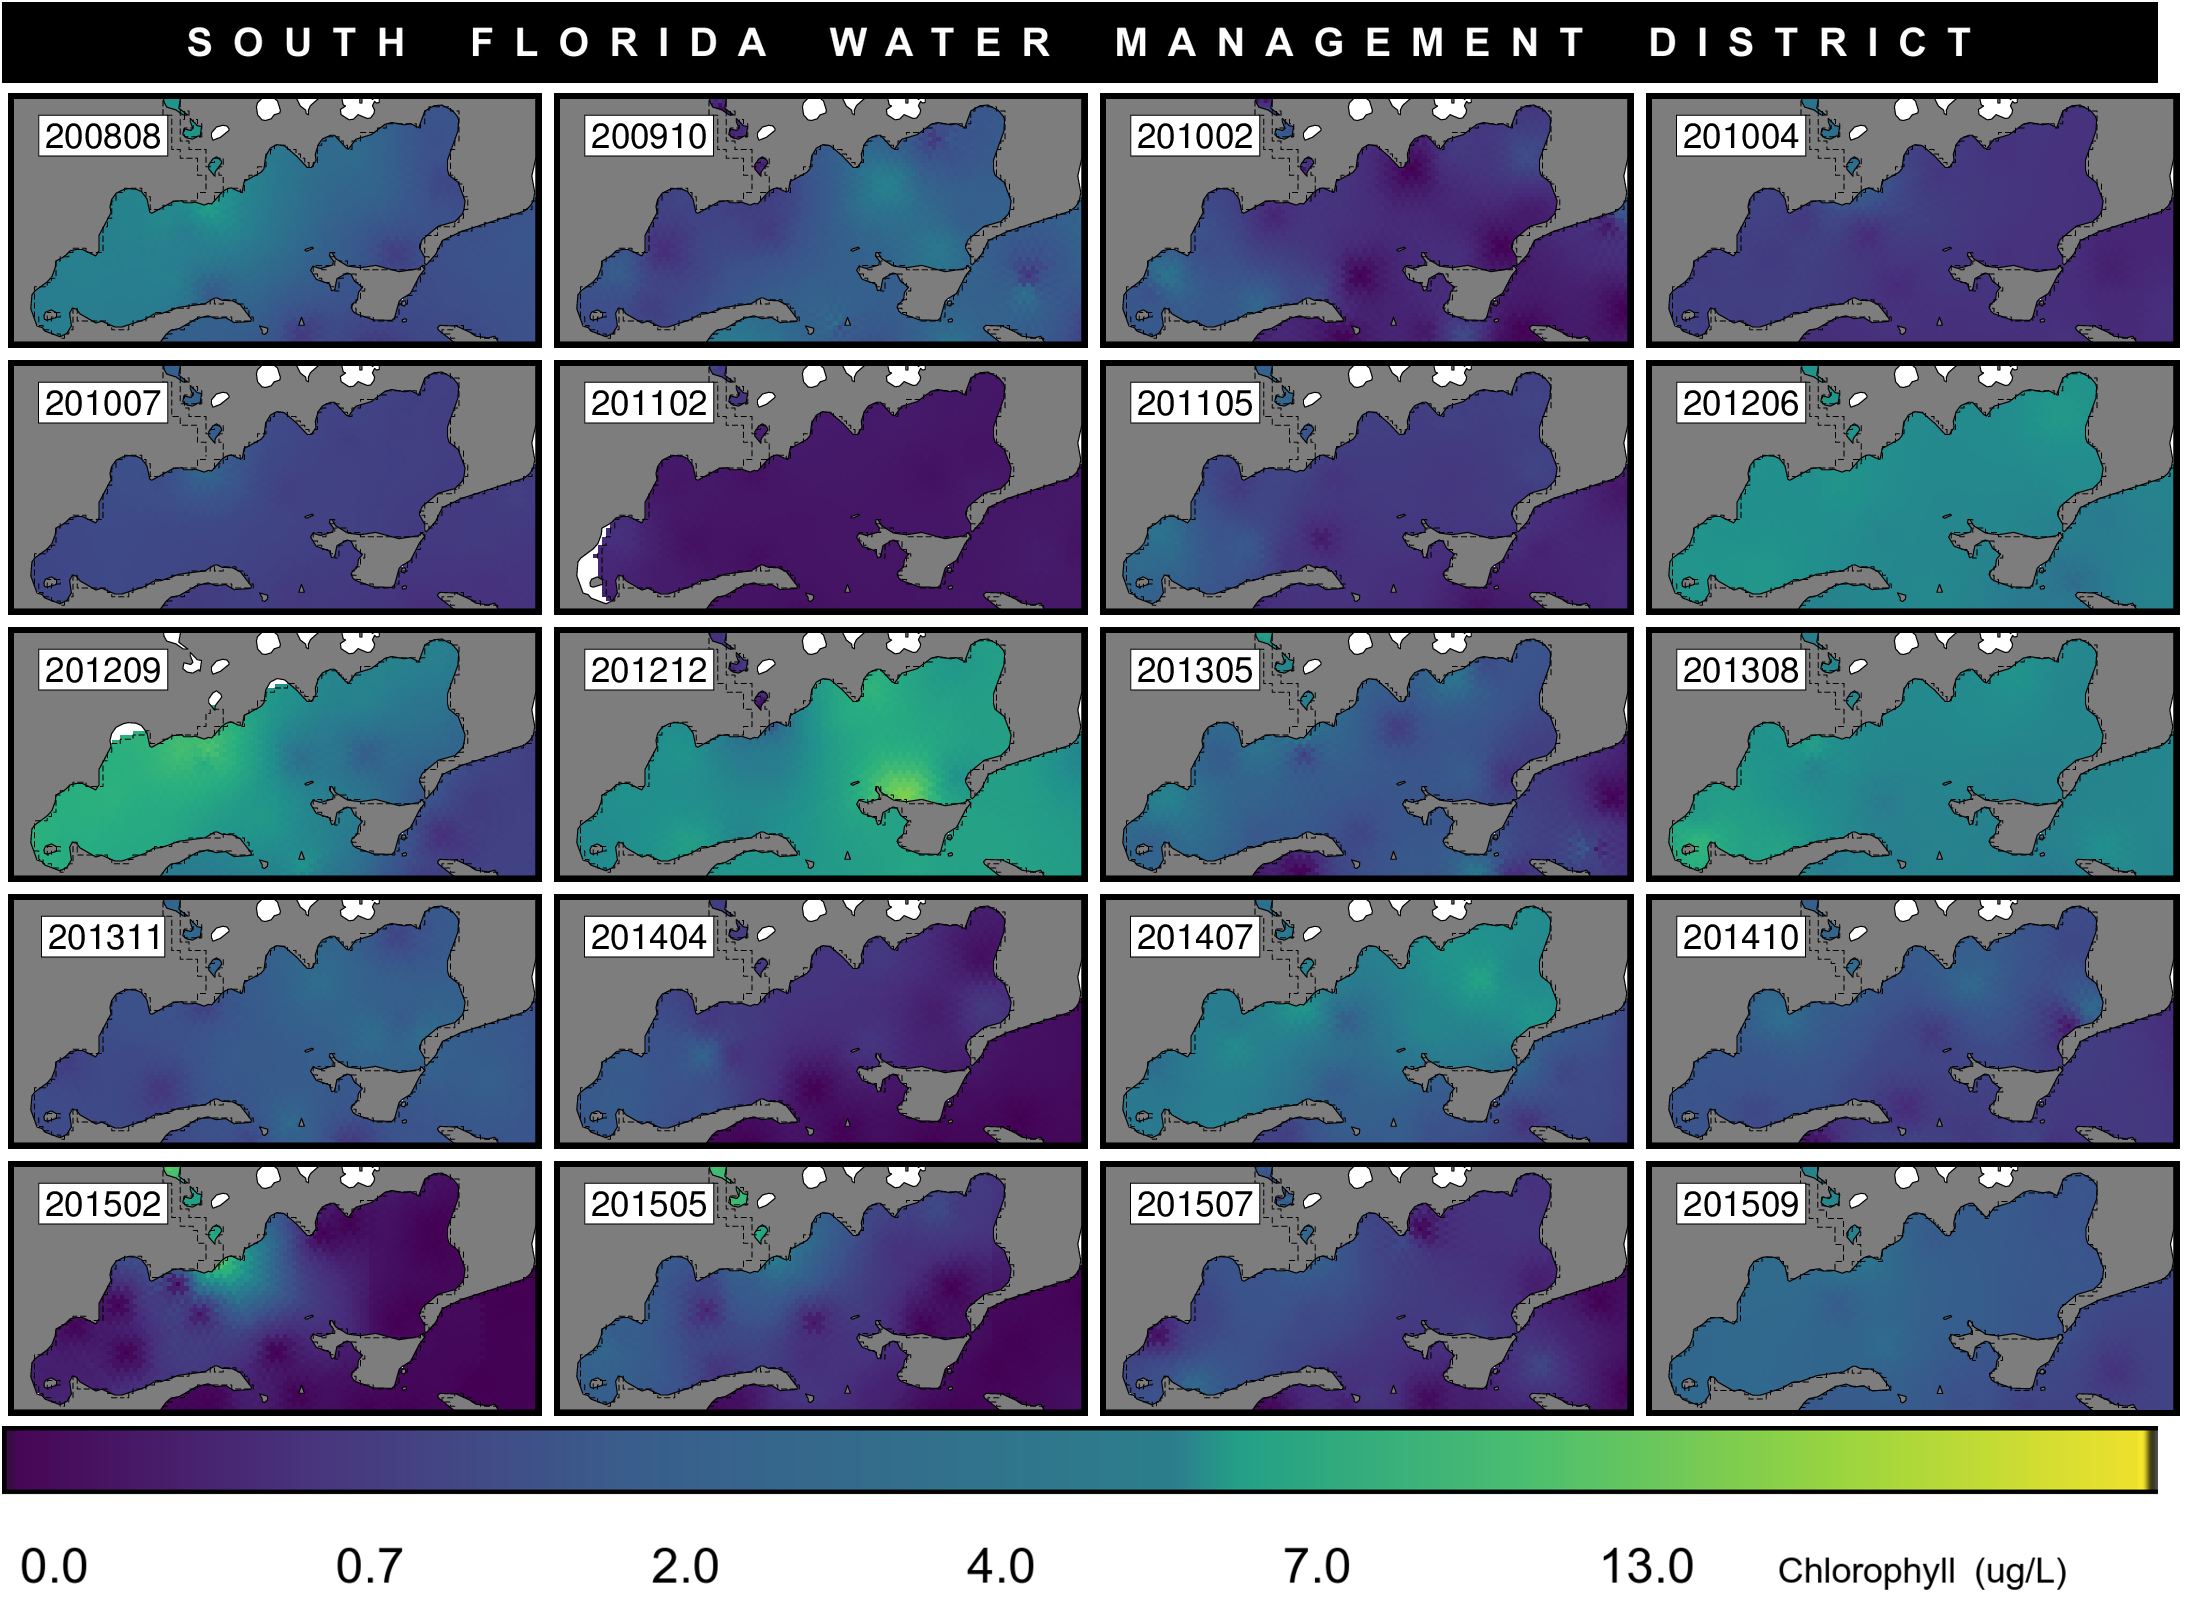
\includegraphics[width=0.75\textwidth]{../../figures/multipanel_mb.png}
  \caption{Chlorophyll concentration in Little Madeira Bay calculated from multiple linear regression using the coefficients in Table 1. Note that the color ramp is log-scaled.}
  \label{fig:a4}
\end{figure*}

\end{document}
% end of file template.tex

